In the previous chapter we introduced the
  core concepts of \lstinline|jsimulation|;
  in the present chapter we delve into \lstinline|jqueues|,
  and explain it center of gravity, viz. {\em (simulation) entities}.
Other fundamental concepts in \lstinline|jqueues|
  like {\em queues\/} and {\em jobs\/},
  both of which are actually specific manifestations of entities,
  are described in subsequent chapters,
  as well as specific implementations of {\em listeners}.
  
Even though this chapter
  is quite abstract
  and deliberately kept compact,
  its contents are crucial for understanding
  core simulation concepts
  like {\em queues\/} and {\em jobs\/}
  in later chapters.
Once you understand entities properly,
  we can describe queues and jobs
  in a highly compact,
  precise and almost mathematical, form.
We therefore strongly recommend to take the time
  to go through this chapter before "jumping into"
  the admittedly more interesting later
  chapters on queues on jobs,
  and to return to this chapter
  if things are unclear later on.
  
\section{Anatomy of a Simulation in \texttt{\bf jqueues}}

Our starting point for a detailed description
  of the \lstinline|jqueues| package,
  is its vision on a {\em simulation run\/};
  a concept already described for \lstinline|jsimulation|
  in Chapter \ref{chap:events-actions-event-list}.
We recall that in a discrete-event simulation,
  the {\em events\/} on an {\em event list\/}
  are processed one at a time
  in order of non-decreasing {\em event time}.
The processing of an event
  involves the invocation of the event's {\em action},
  which in turn may result in the scheduling of new
  events (in the future) on the event list.
A simulation ends when there are no more
  events scheduled on the event list\footnote{
  Or until some other criterion is met;
  see Chapter \ref{chap:events-actions-event-list}.}.

In \lstinline|jqueues|,
  we (have to) narrow this view.
In particular,
  we assume that in a discrete-event simulation (run),
  we are primarily interested in
  a specific subset of objects affected by events.
In \lstinline|jqueues|,
  these objects are called {\em simulation entities}
  and are characterized
  by their implementation of the \lstinline|SimEntity| interface.
There may be many more \lstinline|Java| objects
  that are affected by the scheduled events,
  for instance,
  for logging, reporting or presentation purposes,
  or for statistical analysis,
  or for workload generation,
  but our
  {\em main interest from the problem domain is in the (modeled) entities}.

The crux is that a \lstinline|SimEntity|
  has a well-defined {\em simulation state\/}
  that can change
  {\em only\/} as a result of processing events.
However, these events cannot arbitrarily manipulate
  the state a \lstinline|SimEntity|;
  they can only do so by invoking
  {\em entity operations}.
An operation is a well-defined method, or set of methods,
  on an entity that (potentially) changes its state.
In \lstinline|jqueues|,
  the type use for operations is \lstinline|SimOperation|,
  but you will hardly need this in practical simulations.
Each entity type comes with its specific
  {\em minimal\/} set of admissible operations.
For instance, every queue and job,
  both of which are entities,
  must support the \lstinline|Arrival| operation.

An operation on a \lstinline|SimEntity| is either
  {\em external\/} or {\em internal}.
The former can be scheduled by the end-user,
  whereas the latter can only be scheduled by the entity itself.
For instance,
  for queues, \lstinline|Arrival| is an external operation,
  whereas \lstinline|Departure| is internal.

All entities support the notion of a {\em reset state},
  which is the state\footnote{In the sequel,
  whenever we refer to "the state" of an entity,
  we always mean its "simulation state".}
  they attain upon creation,
  or after a so-called {\em entity reset}.
The reset state is well defined for each entity type;
  for queues, for instance,
  the reset state requirements mandate that the queue is empty.
Performing a reset on an entity is a feature typically needed
  when running a simulation multiple times with the same set of queues
  (or even jobs),
  for instance because a certain accuracy has to be achieved
  (often with {\em variance-reduction\/} techniques like {\em replication\/}).
Because the semantics of an entity reset are rather complicated,
  and many simulation studies do not need it
  (because they simply perform a "single-run"),
  its detailed discussion is deferred.
Nonetheless,
  it is important to realize that every entity
  supports a well-defined reset operation.

Finally, simulation entities are required to
  maintain a set of {\em listeners\/}
  interested in state changes of the entity.
So, whenever the state changes of an entity,
  all of its registered listeners
  are informed.

\begin{figure}[h]
    \label{fig:AnatomyOfASimulationInJQueues}
    \caption{The anatomy of a simulation in \texttt{JQueues}.}
    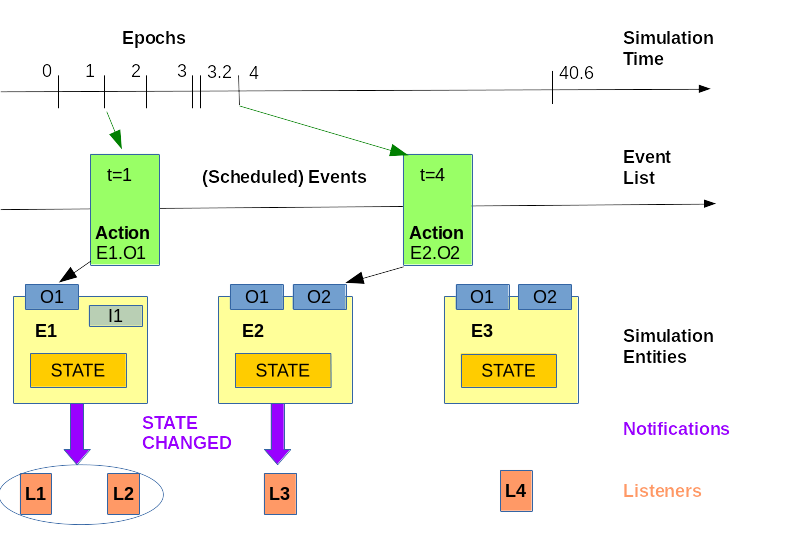
\includegraphics[width=\textwidth]{fig/AnatomyOfASimulationInJQueues}
\end{figure}

In Figure \ref{fig:AnatomyOfASimulationInJQueues},
  we attempt to explain the \lstinline|jqueues|
  concepts and features described thus far.
In the top two rows we show the
  by now hopefully familiar concepts
  of {\em epochs},
  {\em simulation time},
  {\em events},
  and {\em actions}.
The event list contains two events,
  one scheduled at simulation time $t=1$
  and one at $t=4$.
The former's action is to invoke operation
  \lstinline|O1| on entity \lstinline|E1|,
  whereas the latter invokes \lstinline|O2|
  on \lstinline|E2|.
After the effect of invocation of \lstinline|E1.O1|,
  while the event list is being processed,
  entity \lstinline|E1| notifies
  its registered listeners
  \lstinline|L1| and \lstinline|L2|
  through a \lstinline|STATE_CHANGED| notification.
Similarly,
  \lstinline|E2| notifies \lstinline|L3|
  after completing its \lstinline|O2| invocation
  from the event list.
  
\section{The \texttt{\bf SimEntity} Model in More Detail}

In the present section,
  we refine the \lstinline|SimEntity| model
  introduced in the previous section.
In Figure \ref{fig:EntityModel},
  we illustrate the detailed model of a \lstinline|SimEntity|.
We will use this figure in our explanations
  of the more advanced concepts in the next sections.
  
\begin{figure}[h]
    \label{fig:EntityModel}
    \caption{The detailed model of a \texttt{SimEntity}.}
    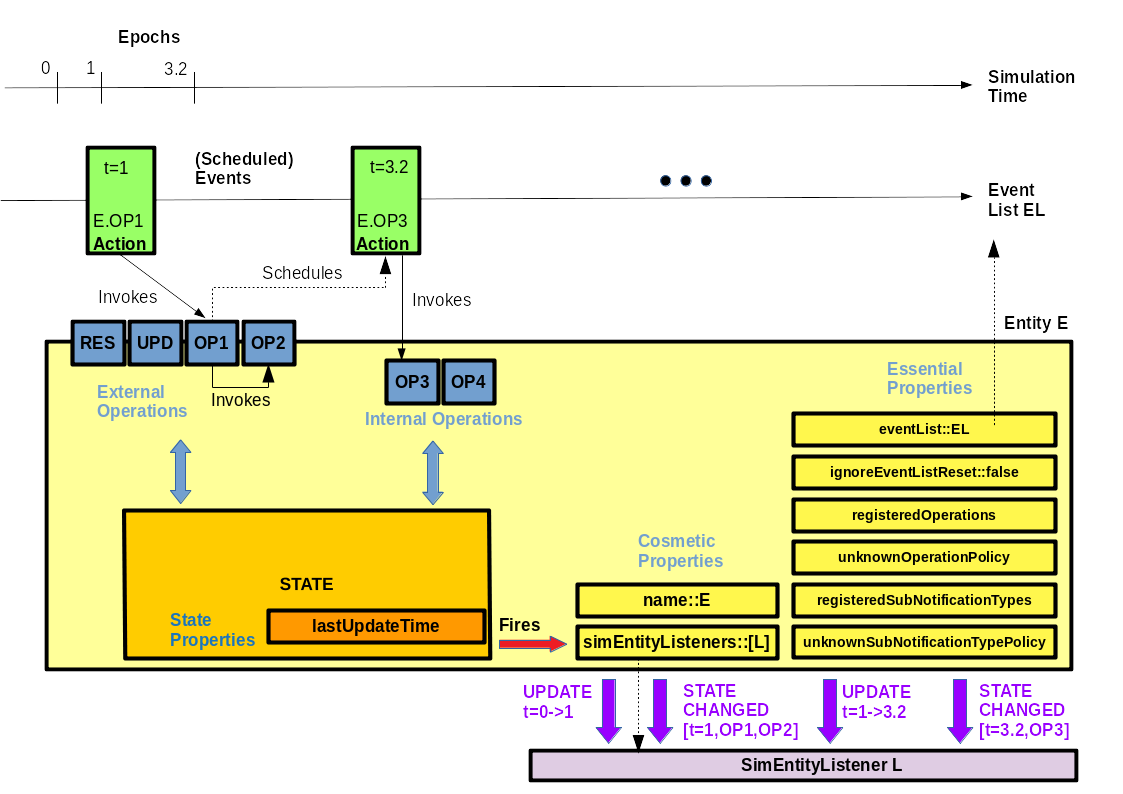
\includegraphics[width=\textwidth]{fig/EntityModel}
\end{figure}

\subsection{Top-Level and Chained Operation Invocations}

When a \lstinline|SimEvent|
  (or, more precisely, its \lstinline|SimEventAction|)
  calls a method on an entity corresponding to one of its operations
  this is called a {\em top-level operation invocation}.
It is perfectly legal for an entity implementation
  to invoke {\em other\/} operations on it
  while performing an operation,
  i.e.,
  still within the context of the event that triggered
  the top-level operation invocation,
  and such invocations are called
  {\em chained operation invocations}.
  
Why is this distinction important?
Well, the golden rule in \lstinline|jqueues|
  is that
  {\em only state changes
       due to top-level operation invocations on an entity
       must be atomically reported to that entity's listeners,
       and only (obviously) after the operation has completed.}
It sounds complicated, but we think it makes more sense
  than to report each individual operation invocation,
  probably exposing an inconsistent state of the entity.

In Figure \ref{fig:EntityModel},
  at $t=1$,
  \lstinline|E.OP1| is invoked from the event list,
  so this invocation is a top-level one.
However,
  {\em while\/} \lstinline|E.OP1| {\em is being processed},
  the entity invokes \lstinline|E.OP2|,
  which is therefore a chained invocation.
It is crucial to understand that
  while \lstinline|E.OP1| also
  schedules the invocation of \lstinline|E.OP3|
  at $t=3.2$,
  the latter when processed will be a top-level invocation
  on its own.
Referring to the lower right part of the figure,
  a listener thus receives a mandatory \lstinline|UPDATE|
  notification at $t=1$,
  indicating a non-trivial progress of time
  (from $t=0$ to $t=1$; we silently assumed that
   the simulation starts at $t=0$)
  without state changes.
It then receives a single \lstinline|STATE_CHANGED|
  notification from the \lstinline|E.O1|
  invocation at $t=1$,
  but notification holds both
  \lstinline|E.O1| and \lstinline|E.O2|
  as sub-notifications,
  because \lstinline|E.O2|
  was invoked from within the
  context of \lstinline|E.O1|.
Their joint effect on the state
  is thus described in a single atomic notification.

\subsection{Top-Level Notifications and Sub-Notifications}

In the previous section
  we learned that entities are obliged to report
  state changes atomically.
On order to avoid potential confusion,
  we need to properly introduce
  some notification-related terminology.
  
A {\em top-level notification\/} is the invocation
  of a method on the registered listeners of an entity.
There exist only the following three types of top-level
  notifications:
\begin{itemize}
\item \lstinline|RESET|:
  The entity has been put into its reset state,
    either because its underlying \lstinline|SimEventList|
    was reset, or because its \lstinline|Reset|
    operation was invoked.
  A \lstinline|RESET| notification is equipped with
    the {\em old\/} time, i.e.,
    the time {\em before\/} the reset,
    and the {\em reset time\/},
    i.e., the {\em new\/} time on the entity\footnote{
    See the description of the \lstinline|lastUpdateTime|
    further in this chapter.}.
  It is important to realize that a \lstinline|RESET|
    notification is the only one allowed to
    "set back" the time on the entity,
    and that it is only issued as a result
    of the invocation of its \lstinline|Reset|
    operation, typically induced from resetting the event list.
  Hence,
    a \lstinline|RESET| notification is {\em not\/}
    issued upon construction of the entity,
    {\em not\/} upon its attachment to a \lstinline|SimEventList|.
\item \lstinline|UPDATE|:
  The entity is {\em about to\/} change its state
    because an operation on it was invoked,
    and it exposes {\em its old state\/}
    and the time at which the update occurs.
  The \lstinline|UPDATE| notification
    primarily targets statistics-gathering listeners
    that need to know the interval length during
    which the entity's state remained constant.
\item \lstinline|STATE_CHANGED|:
  The entity has been subject to the external
    invocation of one of its operations,
    and it exposes its {\em new\/} state
    and the time at which and the manner in which
    the new state was reached.
  The description of the transformation of the old state
    into the new one is done through a sequence
    of {\em sub-notifications\/} described below.
  A \lstinline|STATE_CHANGED| notification
    is not issued when the entity has been reset.
\end{itemize}
Note that there is no dedicated \lstinline|Java| type
  for top-level notifications,
  simply because at the present time,
  we see no purpose in extending
  the current three-sized set of top-level notifications.

A {\em sub-notification\/} is a precise description
  of an aspect of an entity's state transformation.
For the purpose of this description,
  it is always part of a top-level \lstinline|STATE_CHANGED|
  notification.
So, in itself,
  a sub-notification is incomplete.
However, it unambiguously reports
  a state transformation,
  and the state's a priori and a posteriori
  conditions.
So given an entity's state
  (that is valid)
  and a sub-notification,
  one can always predict
  the new state of the entity.
Often,
  it just takes multiple sub-notifications in sequence
  to describe a \lstinline|STATE_CHANGED| notification,
  which explains their existence.
  
A sub-notification is a tuple of its {\em type\/},
  an object implementing \lstinline|SimEntitySubNotificationType|,
  and its arguments.
The actual type of a sub-notification
  defines its required arguments and their structure.
By default,
  a \lstinline|SimEntity| can only emit
  sub-notification types in a \lstinline|STATE_CHANGED|
  notification that have been {\em registered\/}
  at that entity.
The process of registering sub-notification types
  is taken care of in the constructors
  of the various \lstinline|SimEntity|
  sub-types and concrete implementations.
  
\subsection{Properties}

In \lstinline|jqueues|,
  we adopt the notion of object {\em properties\/}
  from \lstinline|JavaBeans|,
  and we silently assume that the reader
  is familiar with the basic concepts
  of \lstinline|JavaBeans|.
We follow the property-naming conventions,
  and in \lstinline|jqueues|,
  we only use property names starting
  with a lower-case letter.

For any \lstinline|SimEntity|,
  we classify its properties as follows\footnote{
  This classification is \texttt{jqueues}-specific;
  it is not part of \texttt{JavaBeans}.}:
\begin{itemize}
\item {\em\bf State Properties\/}
        are part of the entity's simulation state;
        their values can only change as a result of the invocation
        of registered operations on the entity.
      You should never (attempt to) set them directly from user code.
      For a queue, for instance,
        the set of currently visiting jobs
        is a state property.
\item {\em\bf Essential Properties} are {\em not\/} part
        of the entity's simulation state;
        they do, however, affect the
        functionality of an entity's operations,
        {\em and\/} the entity assumes that
        their values {\em remain constant while running a simulation}.
      Hence, 
        their values can only be changed under certain conditions,
        and certainly {\em not\/} (by whatever means)
        {\em while running a simulation}.
      The buffer size of \lstinline|FCFS_B|,
        a \lstinline|FCFS| queueing system with finite buffer space,
        is an example of an essential property,
      because its value decides whether or not an arriving job
        is {\em dropped\/} in the presence of jobs present.
      In other words,
        it affects among others the \lstinline|Arrival| operation.
\item {\em\bf Cosmetic Properties\/} are {\em not\/} part
        of the entity's simulation state,
        but unlike essential properties,
        their values can be changed
        at any time without affecting the simulation state of the entity
        or the functionality of any of its operations.
      Their values may even be changed from an event.
      The name of an entity is a cosmetic property;
        its value, by contract,
        never affect the state of the entity
        nor the functionality of its operations.
\end{itemize}
Note that many sub-types of \lstinline|SimEntity|
  put even stronger restrictions on
  setting an essential property.
In many cases,
  you can only set it {\em upon construction\/},
  or only {\em immediately after a\/} \lstinline|Reset| operation.
  
\section{Mandatory Properties of a \texttt{\bf SimEntity}}

In Table \ref{SimEntity_Properties},
  we list the mandatory properties of a \lstinline|SimEntity|,
  classifying them into state, essential and cosmetic
  properties introduced previously.
  
\begin{table}
\caption{Mandatory properties of a \lstinline|SimEntity|.}
\label{SimEntity_Properties}
\begin{center}
\begin{tabular}{|l|l|l|}
\hline
{\bf Name} & {\bf Type} & {\bf Default/Reset} \\
\hline
\multicolumn{3}{|c|}{} \\
\multicolumn{3}{|c|}{\lstinline[basicstyle=\large]{SimEntity}} \\
\multicolumn{3}{|c|}{} \\
\hline
\multicolumn{3}{|c|}{} \\
\multicolumn{3}{|c|}{\bf State Properties} \\
\multicolumn{3}{|c|}{} \\
\hline
\lstinline|lastUpdateTime| & \lstinline|double| & From \lstinline|eventList|; \\
                           &                    & $-\infty$ if absent. \\
\hline
\multicolumn{3}{|c|}{} \\
\multicolumn{3}{|c|}{\bf Essential Properties} \\
\multicolumn{3}{|c|}{} \\
\hline
\lstinline|eventList| & \lstinline|SimEventList| & From constructor; \\
                      &                          & may be \lstinline|null|. \\
\hline
\lstinline|ignoreEventListReset| & \lstinline|boolean| & \lstinline|false|. \\
\hline
\lstinline|registeredOperations| & \lstinline|Set<SimEntityOperation>|
                                 & Sub-type-dependent; \\
                      &          & set in constructor(s). \\
\hline
\lstinline|unknownOperationPolicy| & \lstinline|UnknownOperationPolicy|
                                   & \lstinline|ERROR|; \\
                        &          & settable by user. \\
\hline
\lstinline|registeredNotificationTypes|
  & \lstinline|Set<Member>|\tablefootnote{In fact,
       \lstinline|SimEntitySimpleEventType.Member|.}
  & Sub-type-dependent; \\
  {\em deprecated}
  & & set in constructor(s). \\
\hline
\lstinline|registeredSubNotificationTypes|
  & \lstinline|Set<SubNotificationType>|
  & Sub-type-dependent; \\
  {\em since r5.3} &          & set in constructor(s). \\
\hline
\lstinline|unknownNotificationPolicy| & \lstinline|UnknownNotificationPolicy|
                                           & \lstinline|ERROR|; \\
{\em deprecated}        &                  & settable by user. \\
\hline
\lstinline|unknownSubNotificationTypePolicy| & \lstinline|UnknownSubNot...Policy|\tablefootnote{
       \lstinline|UnknownSubNotificationTypePolicy|.}
                                          & \lstinline|ERROR|; \\
{\em since r5.3}        &                 & settable by user. \\
\hline
\multicolumn{3}{|c|}{} \\
\multicolumn{3}{|c|}{\bf Cosmetic Properties} \\
\multicolumn{3}{|c|}{} \\
\hline
\lstinline|name| & \lstinline|String| & \lstinline|null|. \\
\hline
\lstinline|simEntityListeners| & \lstinline|List<SimEntityListener>| & Empty \lstinline|List|. \\
\hline
\end{tabular}
\end{center}
\end{table}

The only mandatory state property is \lstinline|lastUpdateTime|
  holding the (a posteriori) simulation time of the last
  (invocation of the) \lstinline|Update|
  or \lstinline|Reset| operation, whichever occurred last.
Note that upon construction,
  a \lstinline|SimEntity| always enters its reset state,
  which sets the initial value of \lstinline|lastUpdateTime|.
This implicit \lstinline|Reset|, however,
  is {\em not\/} notified to listeners
  because there cannot be any.
  
Among the essential properties are
  \lstinline|registeredOperations|
  and
  \lstinline|registeredSubNotificationTypes|,
  reporting the registered operations and notification sub-types,
  respectively.
Typically,
  implementations will return unmodifiable views
  on the underlying collections.
There are also essential properties that govern a
  \lstinline|SimEntity|'s behavior when an
  unregistered operation on it is invoked,
  or when its implementation asks for the emission
  of a sub-notification it does not know.
Both features are of little practical use,
  except perhaps for testing purposes.
Last but not least,
  the \lstinline|simEventList| property holds
  the event list to which the entity is attached.
Typically,
  the event list is passed to the constructor
  of concrete \lstinline|SimEntity| implementations,
  and setting it properly is actually mandatory
  for certain sub-types
  like queues (\lstinline|SimQueue|).
However, {\em if\/} a \lstinline|SimEntity| is attached to a
  \lstinline|SimEventList|,
  the former will register at the latter
  and automatically perform a \lstinline|Reset|
  upon a reset of the event list.
This behavior
  is controlled through the \lstinline|ignoreEventListReset|
  property, but this should {\em never\/}
  be changed by user code; it is strictly meant for
  implementation use.
  
The two mandatory cosmetic properties on a \lstinline|SimEntity|
  are its registered listeners (\lstinline|simEntityListeners|),
  which will be described in more detail in the next section,
  and its \lstinline|name|.
Despite being a "cosmetic" property,
  setting the \lstinline|name|
  of a \lstinline|SimEntity|
  is often quite important.
Typically,
  if you do not set it,
  implementations of \lstinline|SimEntity|
  will use a {\em type-specific\/}
  \lstinline|String|
  for the \lstinline|toString| method;
  otherwise,
  they will supply the value of the \lstinline|name|
  property.
So,
  if you are studying a single queue like \lstinline|FCFS|,
  there is really no need to set its name;
  its default \lstinline|toString| representation
  will be \lstinline|"FCFS"|,
  which is clear enough.
If, however,
  you use multiple queues of the same type,
  or if distinct individual identification is required
  of the {\em jobs\/} (\lstinline|SimJob|)
  the queue(s) is/are subject to,
  it is highly recommended to set the
  \lstinline|name| property accordingly.
(Another, implementation-driven argument for this approach
  is that end users can set an entity's name
  {\em even if the implementation is final}.
On such implementations,
  one clearly cannot override \lstinline|toString|.)
  
\section{Registering and Unregistering Listeners}

As stated previously,
  a \lstinline|SimEntity| must always report state changes atomically
  to each registered listener.
In \lstinline|jqueues|,
  such listeners have type \lstinline|SimEntityListener|,
  and they can be registered and
  unregistered at any time on a \lstinline|SimEntity|
  through the \lstinline|registerSimEntityListener|
  and \lstinline|unregisterSimEntityListener|
  methods, respectively.
The set of currently registered listeners of an entity
  is available through its \lstinline|simEntityListeners| property,
  which is a cosmetic property and
  thus {\em not\/} part of the entity's state.
  
\section{Mandatory Operations on a \texttt{\bf SimEntity}}

Every \lstinline|SimEntity| {\em must\/} support the following operations,
  all of which are {\em external\/}:
\begin{itemize}
\item \lstinline|Reset|: This operation puts the entity into its reset state,
                           and sets its \lstinline|lastUpdateTime| property
                           to the time argument provided.
                         It is the {\em only\/} operation allowed to
                           "set back" the time on the entity.
                         The \lstinline|RESET| operation is not meant
                           to be invoked directly from user code.
                         If the \lstinline|SimEntity| is attached to an
                           event list, through its \lstinline|simEventList| property,
                           it will reset itself automatically when the
                           attached event list resets.
                         A \lstinline|SimEntity| will issue
                           a \lstinline|UPDATE| notification first
                           when its \lstinline|Reset| operation is (explicitly) invoked,
                           and after completion, it will notify its listeners
                           with a \lstinline|RESET| notification.
                         Upon construction,
                           a \lstinline|SimEntity| always enters its reset state,
                           possibly overriding state-property values
                           (directly or indirectly) from the
                           constructor arguments.
                         This is an implicit invocation of \lstinline|Reset|
                           which is not reported to listeners.
\item \lstinline|Update|: This operation sets the \lstinline|lastUpdateTime|
                            property on the entity from the time argument supplied,
                            and notifies listeners through the \lstinline|UPDATE|
                            notification,
                            providing both a priori and a posteriori simulation time.
                          It {\em never\/} modifies state properties other than
                            \lstinline|lastUpdateTime|.
\item \lstinline|DoOperation|: This "meta operation" invokes the operation
                                 provided as argument.
                               The operation has to be registered at the
                                 \lstinline|SimEntity|; if not
                                 the behavior of the entity is controlled
                                 by the value of its
                                 \lstinline|unknownOperationPolicy| property.
                               The operation-specific arguments have to be provided
                                 as well.
\end{itemize}

\section{Summary}

In this chapter, we introduced the core concept of \lstinline|jqueues|,
  viz., \lstinline|SimEntity|s.
Below, we summarize the contents of this chapter:
\begin{itemize}
\item In \lstinline|jqueues|,
        we are primarily interested in the behavior in simulation time
        of objects named {\em (simulation) entities}.
\item Simulation entities model objects from the real-world
        problem domain; they are represented as \lstinline|SimEntity|
        \lstinline|Java| objects.
      Queues and jobs are typically instantiations of entities.
\item A \lstinline|SimEntity| has a well-defined
        {\em simulation state\/},
        which is a subset of the \lstinline|Java|
        object state.
      The simulation state can only change as a result
        of the invocation of registered \lstinline|SimOperation|s
        on the entity.
\item The invocation of an operation on a \lstinline|SimEntity|
        from the event list is called a {\em top-level operation invocation}.
      Such invocation may induce the invocation of other operations
        on the \lstinline|SimEntity|; these are called {\em chained invocations}.
\item A \lstinline|SimEntity| processes and reports its
        top-level operation invocations {\em atomically}.
      The reports of state changes are through \lstinline|STATE_CHANGED|
        notifications, which consists of a sequence of {\em sub-notifications\/}
        each describing a specific, well-defined, transformation of
        the entity's state.
\item Like operations, sub-notifications need to be of a known type,
        well documented,
        and registered at the \lstinline|SimEntity|.
\item A \lstinline|SimEntity| exposes its \lstinline|Object|
        state through \lstinline|JavaBeans| properties.
      A property can be a {\em state\/} property,
        representing an aspect of the entity's simulation state,
        a {\em essential\/} property,
        having dominant effect on the behavior of operations,
        or a {\em cosmetic\/} property,
        which does {\em not\/} have that effect.
\item Each \lstinline|SimEntity| must support the
        \lstinline|Reset|, \lstinline|Update|
        and \lstinline|DoOperation| operations.
\item Each \lstinline|SimEntity| must support the
        \lstinline|RESET|, \lstinline|UPDATE|
        and \lstinline|STATE_CHANGED| top-level notifications.
\end{itemize}